\section{Istruzione per l'utilizzo}
  L'header della {dashboard}\ped{G} è uguale come struttura per ogni tipo di utente. Su di esso troviamo un link che porta alla modifica dei dati personali, chiamato \textit{Profilo}, e un link, \textit{Esci}, che, se cliccato, effettua il logout dal sistema.



\subsection{Interfaccia}
    \begin{figure}[H]
        \centering
   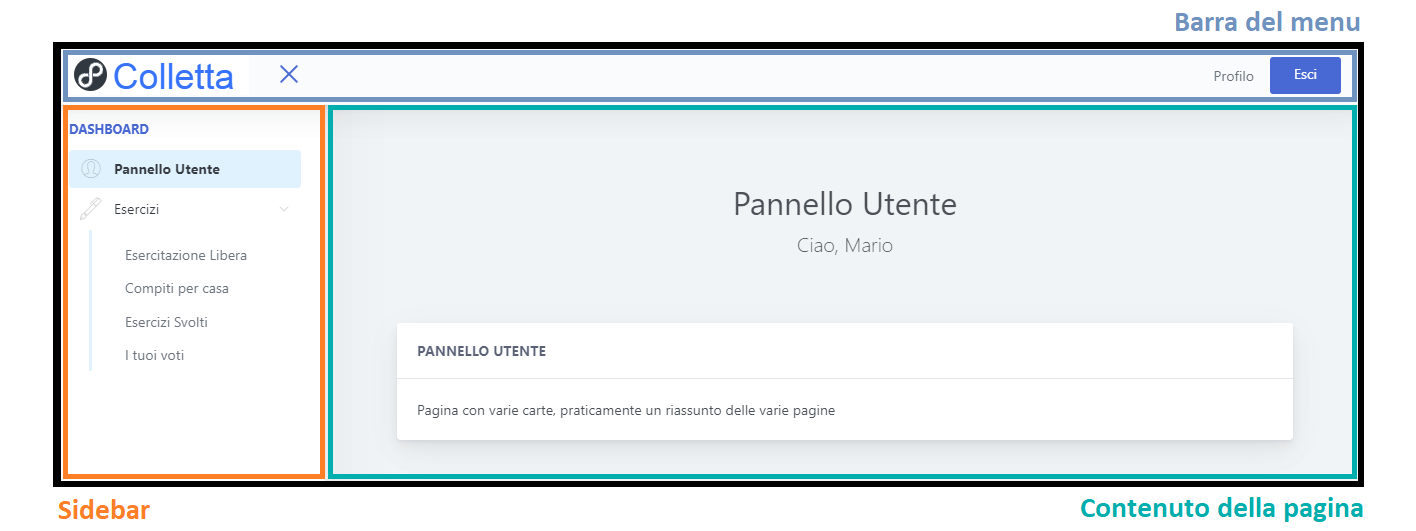
\includegraphics[width=17cm]{sez/img/istruzioni/panoramica.png} 
        \caption{Panoramica dell'interfaccia}\label{fig:1}
    \end{figure}
  La struttura generale di una pagina è la stessa per ogni utente loggato. Sono presenti i seguenti elementi di base:
    \begin{itemize}
        \item Barra del menu;
        \item {Sidebar}\ped{G};
        \item Contenuto della pagina.
    \end{itemize}
 A seconda del tipo di utente (Allievo, Insegnante, Sviluppatore, Amministratore) e della pagina selezionata, verranno visualizzati a schermo contenuti diversi. Ogni utente ha comunque a disposizione lo stesso header e un link al suo pannello utente.


\subsection{Utente non autenticato}
    \subsubsection{Registrazione}
    	\begin{figure}[H]
        	\centering
        	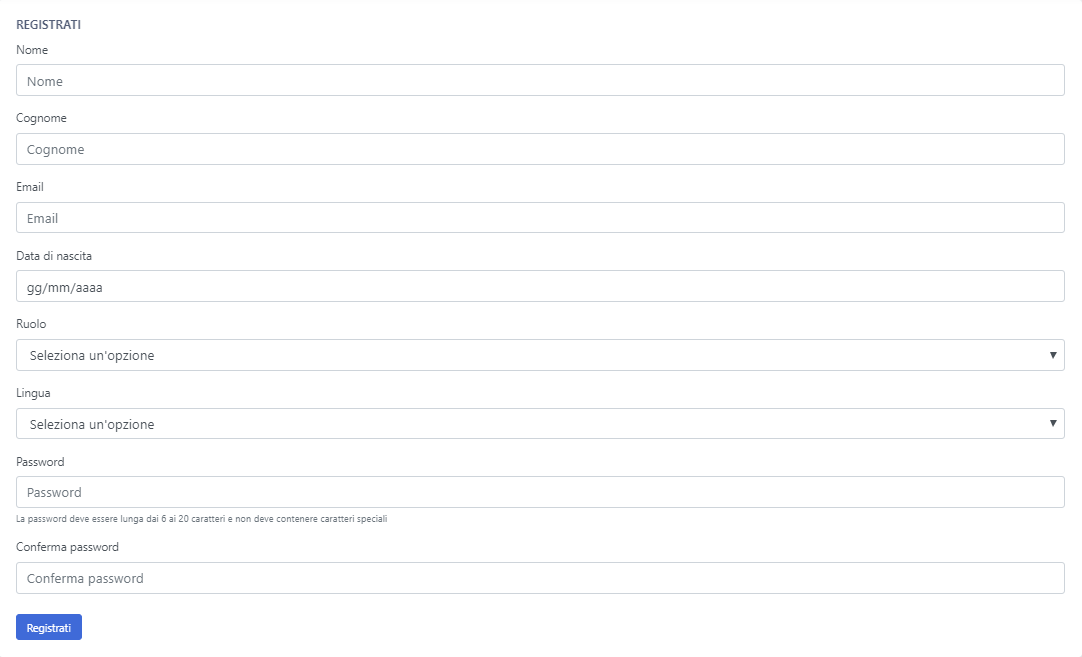
\includegraphics[width=1\linewidth]{sez/img/autenticazione/formRegistrazione.PNG} 
        	\caption{Form per la registrazione}\label{fig:registrazione}
    	\end{figure}
	  Se non si è ancora registrati è possibile farlo cliccando sul bottone \textit{Registrati} presente nella barra del menu. Una volta compilato il form sarà possibile accedere alla piattaforma come utente autenticato. Se si sceglie come ruolo \textit{sviluppatore} sarà necessario attendere una conferma da parte dell'amministratore prima di poter accedere. I dati sono tutti obbligatori e il form visualizzato sarà quello in \autoref{fig:registrazione}.\\
	  Dopo la registrazione, si verrà automaticamente loggati nel profilo appena creato, eccetto nel caso in cui l'utente si sia registrato come sviluppatore.
    \subsubsection{Login}
    	\begin{figure}[H]
        	\centering
        	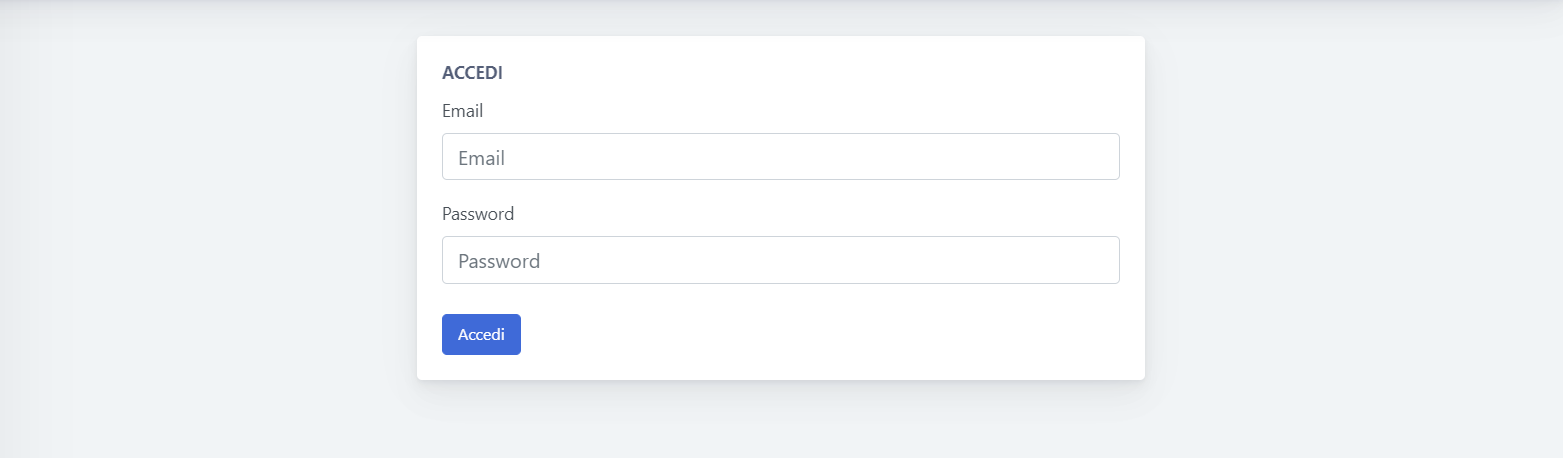
\includegraphics[width=1\linewidth]{sez/img/autenticazione/formAccedi.PNG} 
        	\caption{Dati per effettuare l'accesso}\label{fig:1}
    	\end{figure}
 	  Dopo aver effettuato la registrazione si accede cliccando su \textit{Accedi} nella barra del menu. Si accede inserendo email e password.


% UTENTE AUTENTICATO
\subsection{Utente autenticato generico}

    \subsubsection{Logout}
    Per effettuare il {logout}\ped{G} si deve cliccare sulla voce \textit{Esci} dalla barra del menu. Facendo ciò, l'utente termina la propria sessione.
    \subsubsection{Modifica dati}
    Cliccando su \textit{profilo} l'utente ha la possibilità visualizzare e modificare i propri dati tramite un form simile a quello di registrazione. L'utente non può modificare il proprio ruolo e la propria Email dopo l'iscrizione.

    \subsection{Allievo}
      L'allievo si iscrive nel portale Colletta per svolgere esercizi di analisi grammaticale. Può svolgere esercizi assegnati da un'insegnante o svolgere esercizi liberi tramite il sistema di correzione automatica del sistema. L'allievo ha poi la possibilità di confrontare la sua soluzione con quella presentata dal sistema.
        \subsubsection{Sidebar}
          La sidebar dell'allievo presenta le seguenti voci:
            \begin{itemize}
                \item Pannello utente;
                \item Esercitazione libera;
                \item Compiti per casa;
                \item Esercizi svolti.
            \end{itemize}
            

            
        \subsubsection{Pannello utente}
          Il pannello utente è un riassunto di tutti i progressi e le attività svolte dall'allievo. Al momento il pannello utente mostra un messaggio di benvenuto, l'allievo è quindi libero di selezionare una delle voci di menu ed esercitarsi.
%        	\begin{itemize}
%        		\item Progressi;
%        		\item Traguardi;
%        		\item Traguardo corrente;
%        		\item Prossimo traguardo;
%        		\item Valutazioni;
%        		\item Esercizi recenti;
%        		\item Insegnanti preferiti.
%        	\end{itemize}
        
        
               
	\newpage
        \subsubsection{Esercitazione libera}      
        	\begin{figure}[H]
                \centering
                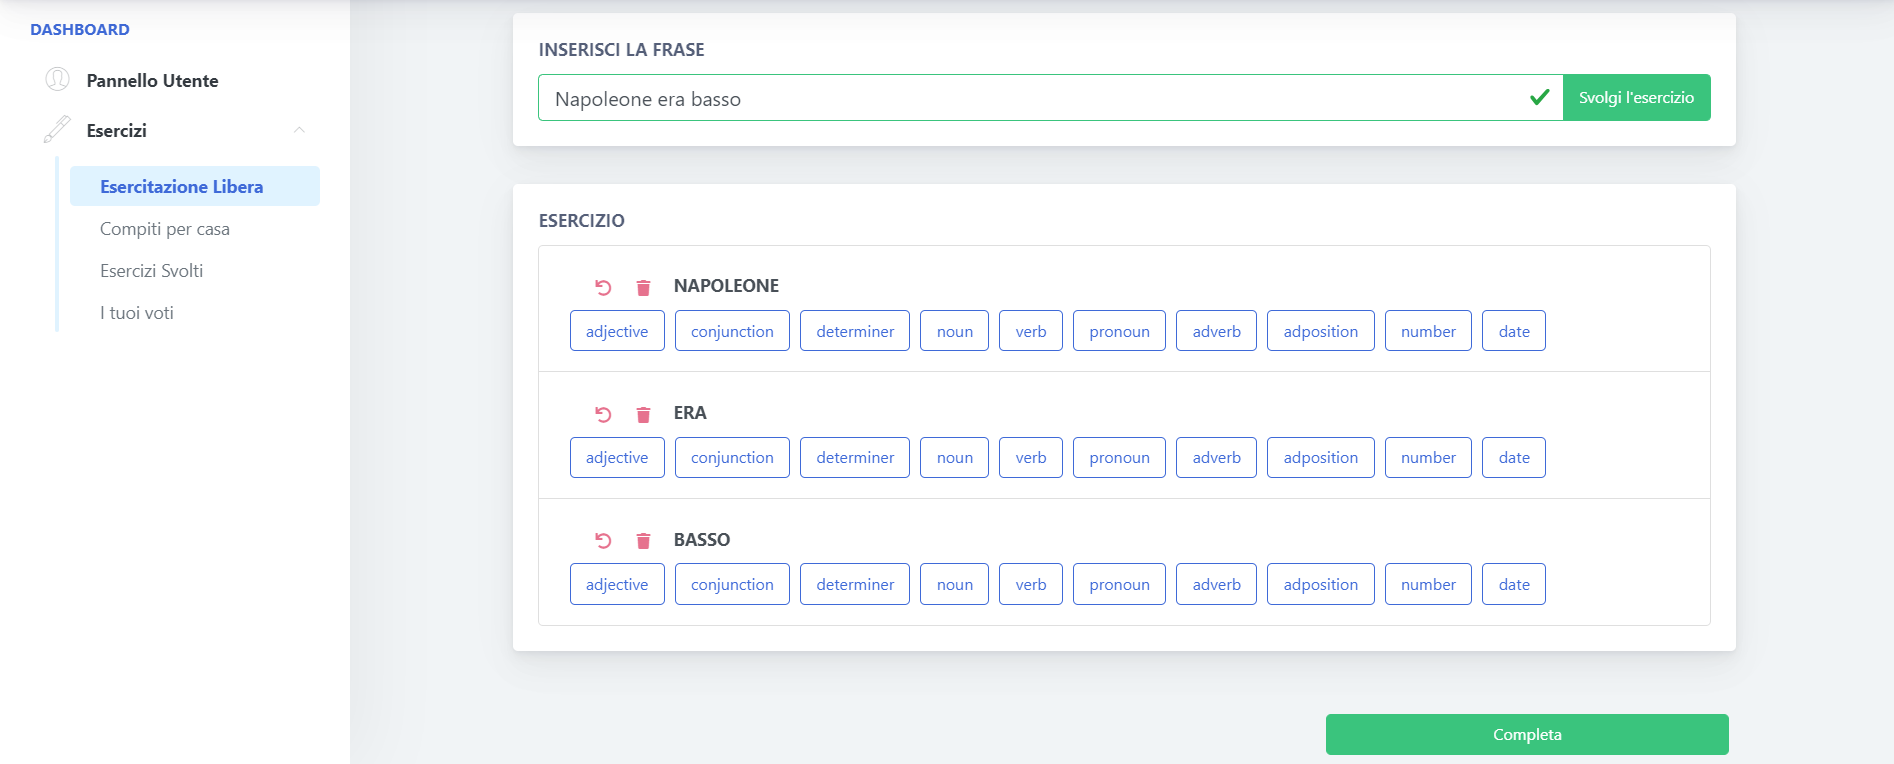
\includegraphics[width=17cm]{sez/img/studente/esercitazioneLiberaEsegui.PNG} 
                \caption{Svolgimento esercizio libero}\label{fig:1}
        	\end{figure}
          In questa pagina è possibile svolgere un esercizio inserendo nella casella di testo una frase da analizzare.
          Se la frase non è stata inserita da nessun insegnante la correzione sarà generata automaticamente.\\
        \\ Svolgimento:
        	\begin{enumerate}        
            	\item Scrivere la frase da analizzare dentro al form;
            	\item Cliccare su \textit{Svolgi l'esercizio};
            	\item Svolgere l'esercizio e cliccare \textit{Completa}.
        	\end{enumerate}
        	\label{sec:esLib}
        	Lo svolgimento dell'esercizio è guidato da dei bottoni che aiutano l'allievo a eseguire un'analisi precisa. Ogni parola presenta dei bottoni sottostanti che rappresentano le scelte disponibili: cliccandoci sopra, il testo del bottone verrà aggiunto alla soluzione, e verrà mostrato un nuovo set di bottoni con ulteriori opzioni per l'analisi. In caso non comparissero più pulsanti, significa che l'analisi per quella parola è terminata. In ogni momento, l'allievo può decidere di resettare la soluzione per una determinata parola (icona cestino), o annullare l'ultima scelta (freccia indietro).

      
        \newpage
  		\subsubsection{Compiti per casa}
 		  In questa sezione l'allievo ha la possibilità di visualizzare gli esercizi a lui assegnati, scegliendo di svolgere uno qualsiasi fra gli esercizi elencati.
        	\begin{figure}[H]
            	\centering
            	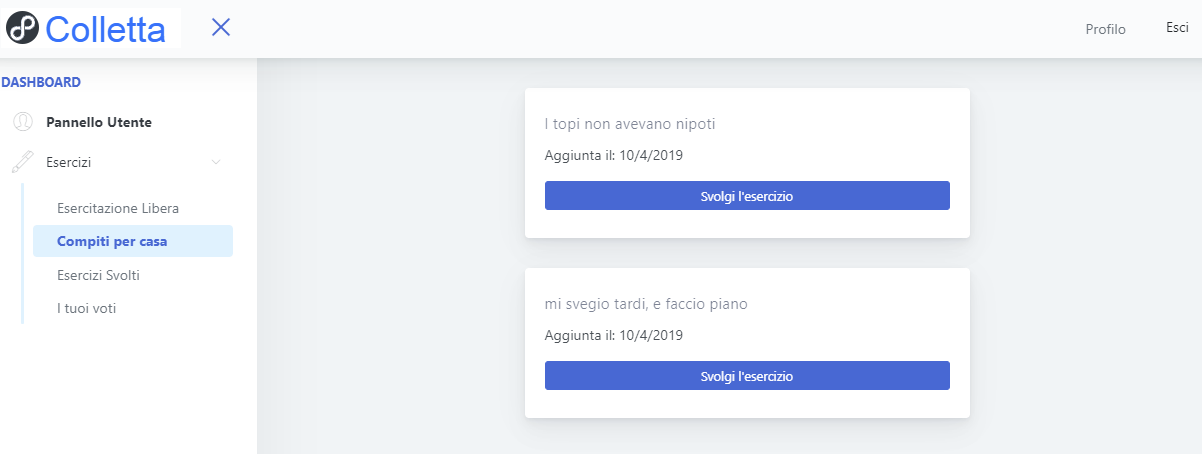
\includegraphics[width=17cm]{sez/img/studente/compitopercasa.PNG} 
            	\caption{Scelta esercizio da risolvere}\label{fig:1}
        	\end{figure}

		  L'allievo sceglie l'esercizio da svolgere tra quelli che sono stati assegnati cliccando su \textit{Svolgi l'esercizio}.   
       
        	\begin{figure}[H]
            	\centering
            	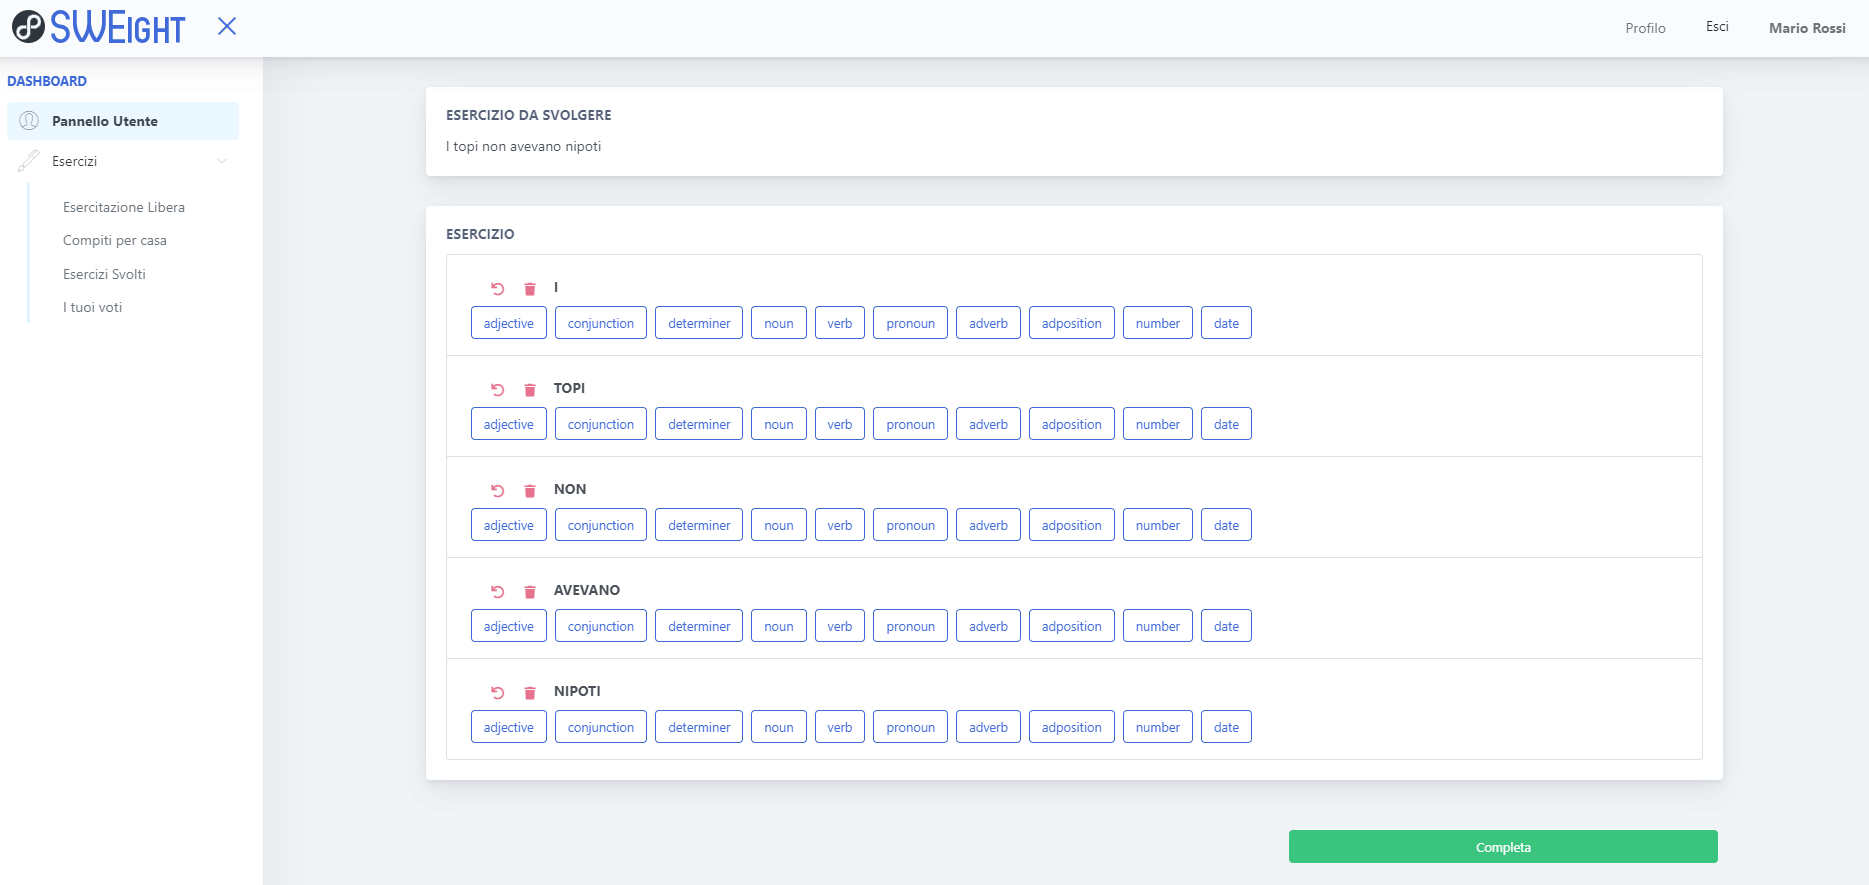
\includegraphics[width=17cm]{sez/img/studente/svolgimentoesercizio.PNG} 
            	\caption{Svolgimento esercizio}\label{fig:1}
        	\end{figure}      
	L'allievo esegue quindi l'analisi della frase allo stesso modo descritto in \S\ref{sec:esLib}. La soluzione visualizzata alla fine sarà in questo caso quella dell'insegnante che ha assegnato l'esercizio.
        
        
        
        \subsubsection{Esercizi svolti}
        	\begin{figure}[H]
            	\centering
            	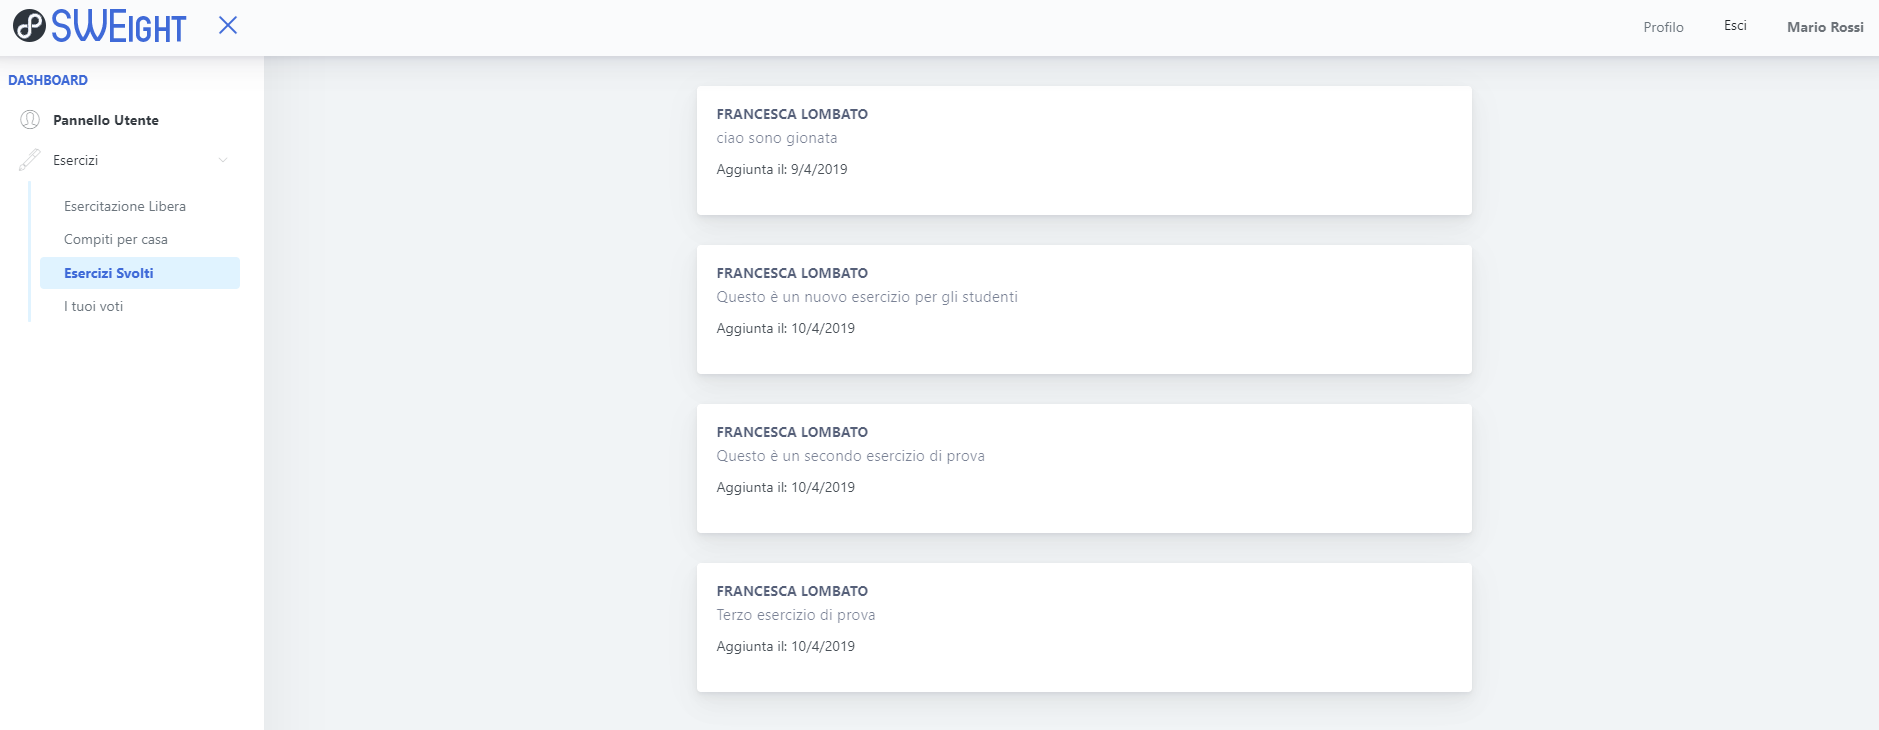
\includegraphics[width=17cm]{sez/img/studente/esercizisvolti.PNG} 
            	\caption{Storico esercizi svolti}\label{fig:1}
        	\end{figure}
          In questa pagina è possibile visualizzare lo storico degli esercizi che sono stati svolti. Per ogni esercizio svolto sono visualizzabili la data di aggiunta, la frase analizzata e il nome dell'insegnante che ha assegnato l'esercizio.
        
\newpage
    \subsection{Insegnante}
      L'insegnante è l'utente che può inserire esercizi privati o decidere di assegnarli ai propri allievi. 
        \subsubsection{Sidebar}
          La sidebar dell'insegnante presenta le seguenti voci:
        	\begin{itemize}
            	\item Pannello utente;
            	\item Inserisci esercizio;
            	\item Esercizi inseriti;
            	\item Esercizi allievi.
        	\end{itemize}
        
        
        
        \subsubsection{Pannello utente}
          Il pannello utente mostra un messaggio di benvenuto all'insegnante, che poi è libero di spostarsi sulla sidebar e assegnare esercizi ai propri allievi.
        
        
        \subsubsection{Inserisci esercizio}
          Questa sezione da la possibilità all'insegnante di inserire un esercizio nel sistema.
        	\begin{figure}[H]
            	\centering
        		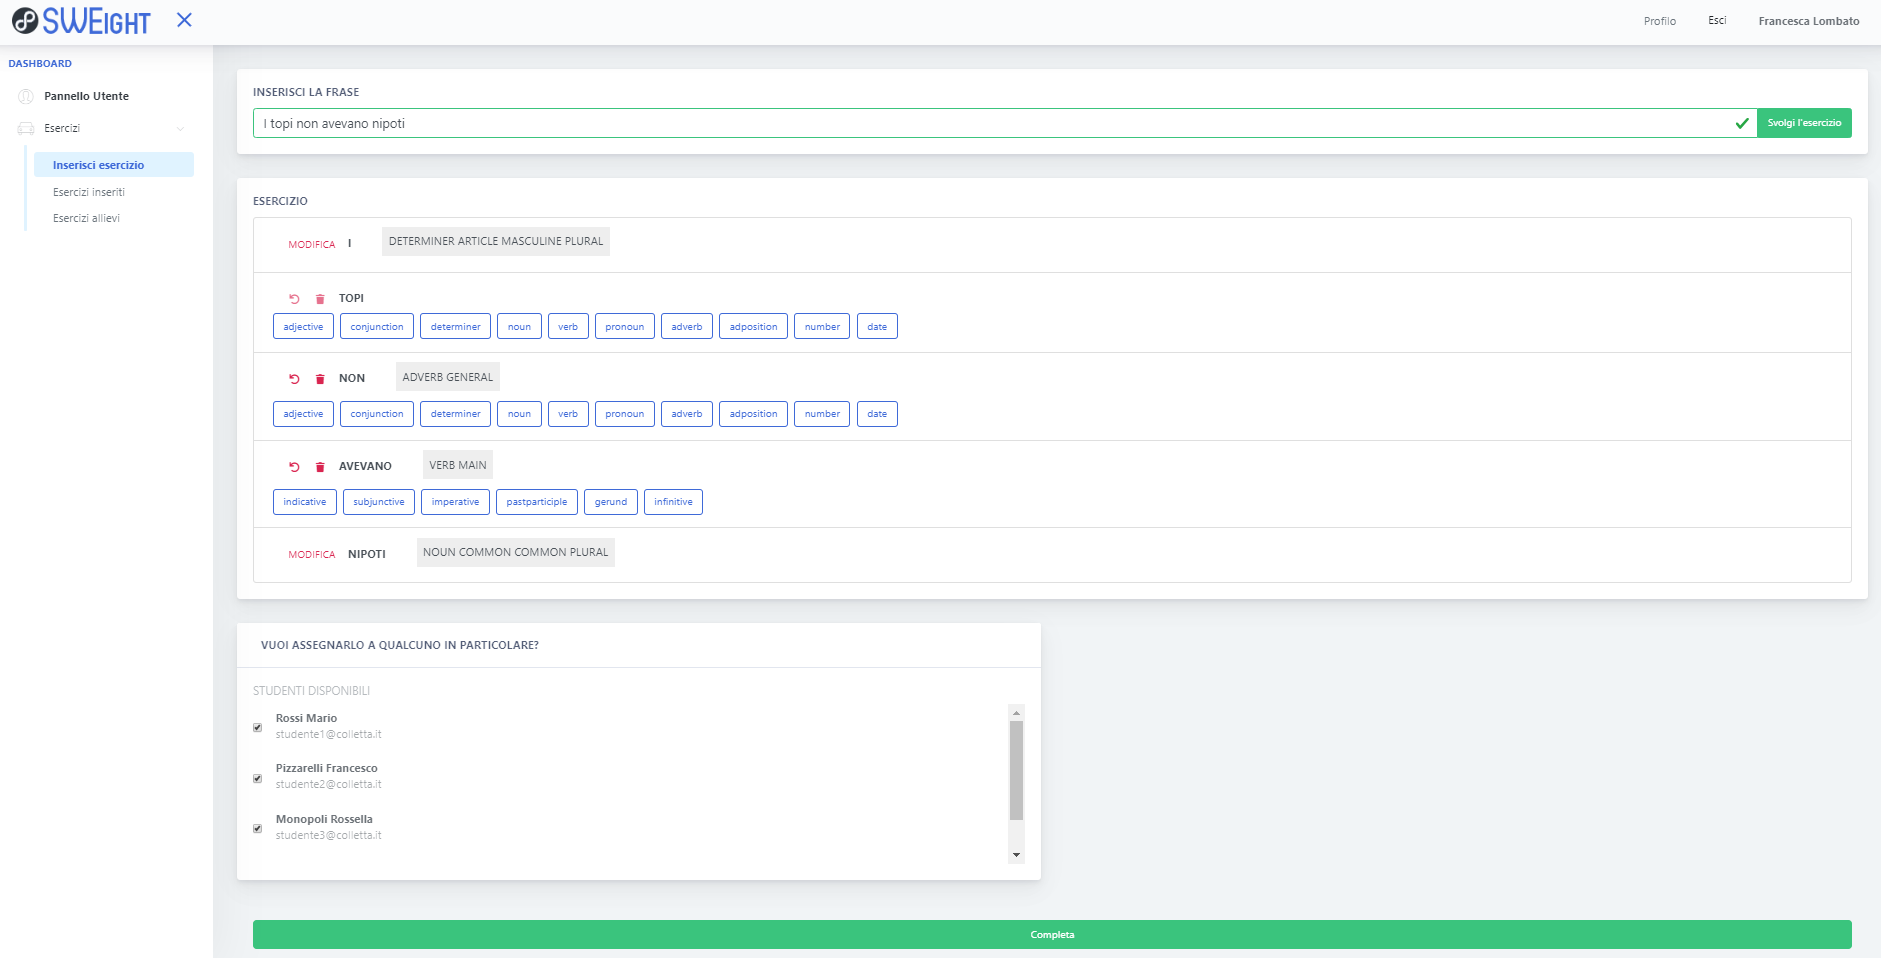
\includegraphics[width=17cm]{sez/img/insegnante/inserisciEsercizio.PNG} 
            	\caption{Inserimento e assegnazione esercizio}\label{fig:1}
        	\end{figure}
        
          Dopo aver inserito la frase, verrà visualizzata la correzione automatica. Se ritenuta errata c'è la possibilità di modificare la soluzione cliccando su \textit{Modifica}. Durante lo svolgimento dell'esercizio l'insegnante ha la possibilità di tornare indietro di un passo, o di resettare completamente la soluzione per ogni parola. Questo processo è analogo a quello presentato in \S\ref{sec:esLib}. Finita la correzione, l'insegnate ha la possibilità di assegnare l'esercizio a un allievo e cliccando \textit{Completa} esso verrà aggiunto nel database.
        
        
        
        \subsubsection{Esercizi inseriti}
        
        Funzionalità al momento non disponibile. Questa sezione permette di visualizzare tutti gli esercizi inseriti, si possono vedere la frase inserita e la data di aggiunta.
        
        
        
        
        \subsubsection{Esercizi allievi}        
         Funzionalità al momento non disponibile. In questa sezione sono visibili i risultati dagli allievi.
        
        
        
        
	\newpage
    \subsection{Sviluppatore}
    Lo sviluppatore si iscrive al sito perchè interessato a scaricare i dati prodotti dagli utenti durante l'esecuzione di esercizi di analisi grammaticale.
    	\subsubsection{Sidebar} 
    	  La sidebar dello sviluppatore presenta le seguenti voci:
    		\begin{itemize}
    			\item Pannello utente;
    			\item Pannello sviluppatore.
    		\end{itemize}
    
    
    
    
    	\subsubsection{Pannello utente}
    	  Il pannello utente mostra un messaggio di benvenuto allo sviluppatore, che è libero di procedere allo scaricamento dei dati prodotti dagli utenti.



    	\subsubsection{Pannello sviluppatore}
    		\begin{figure}[H]
				\centering
				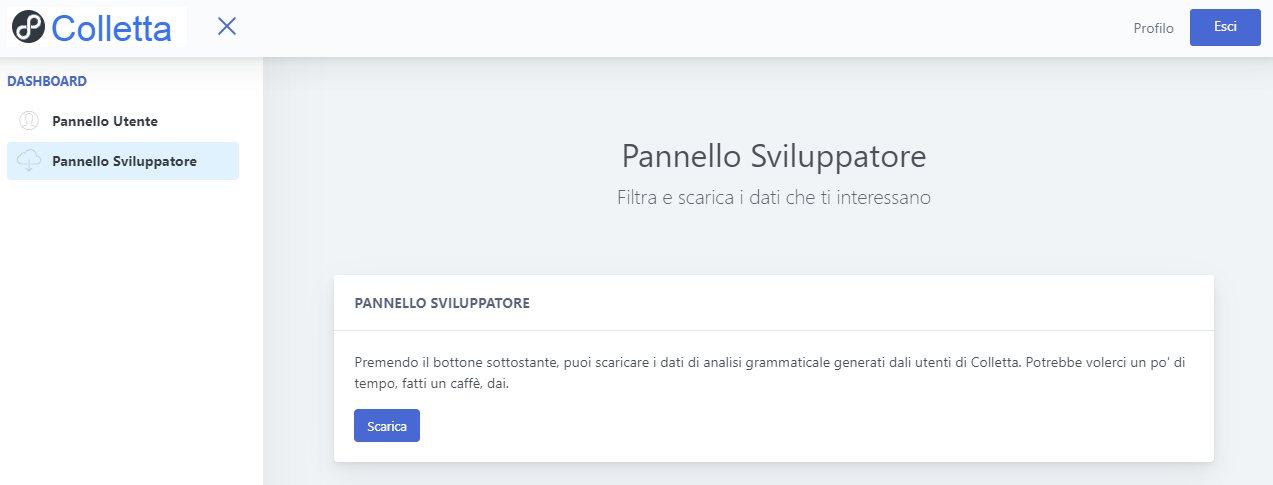
\includegraphics[width=17cm]{sez/img/sviluppatore/datipronti.png}
				\caption{Scaricamento dati disponibili}\label{fig:1}
			\end{figure}
		  Cliccando sul bottone di \textit{Scarica}, lo sviluppatore può scaricare i dati prodotti dagli utenti, avrà successivamente la possibilità di filtrare questi dati.




	\newpage
	\subsection{Amministratore}
	L'amministratore ha la possibilità di gestire tutti gli utenti che non siano amministratori; inoltre può approvare o declinare le richieste di iscrizione degli sviluppatori.
		\subsubsection{Sidebar}
		  Voci nella sidebar:
			\begin{itemize}
				\item Pannello utente;
				\item Sviluppatori;
				\item Utenti.
			\end{itemize}



		\subsubsection{Pannello utente}
		 Il pannello dà il benvenuto allo sviluppatore, che è libero di procedere alla gestione degli utenti.




		\subsubsection{Sviluppatori}
			\begin{figure}[H]
				\centering
				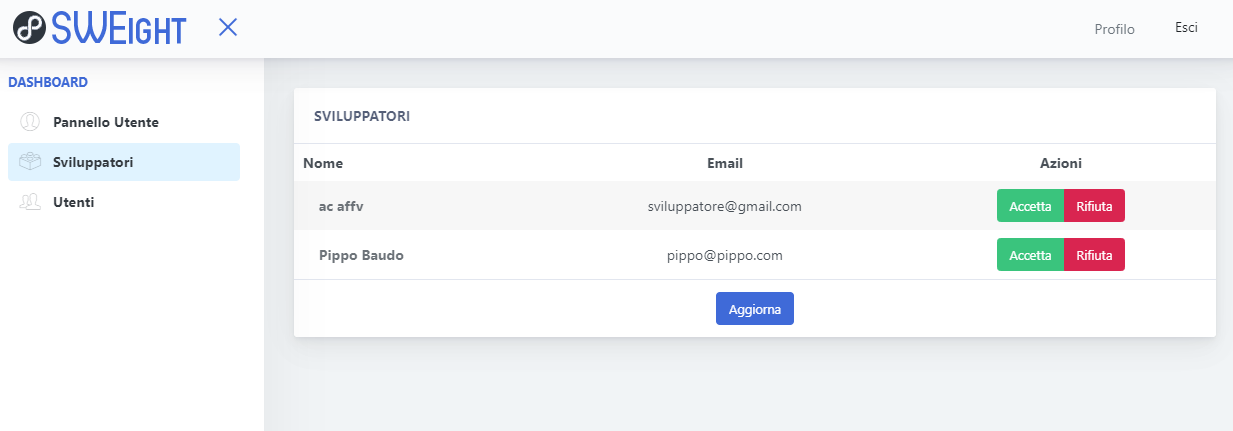
\includegraphics[width=17cm]{sez/img/amministratore/conf_ric_svil.PNG}
				\caption{Richieste di iscrizione degli sviluppatori}\label{fig:1}
			\end{figure}
		  In questa pagina l'amministratore può approvare o rifiutare le richieste di iscrizione degli sviluppatori. Viene presentata una lista contente gli sviluppatori che hanno richiesto di iscriversi al sistema. Ogni sviluppatore ha un nome e una mail. L'amministratore, premendo su \textit{Accetta}, consente allo sviluppatore di fare il login; se invece preme su \textit{Rifiuta}, l'amministratore cancella lo sviluppatore dal sistema. Premendo su \textit{Aggiorna}, l'amministratore aggiorna la lista di sviluppatori.


		\subsubsection{Utenti}
			\begin{figure}[H]
				\centering
				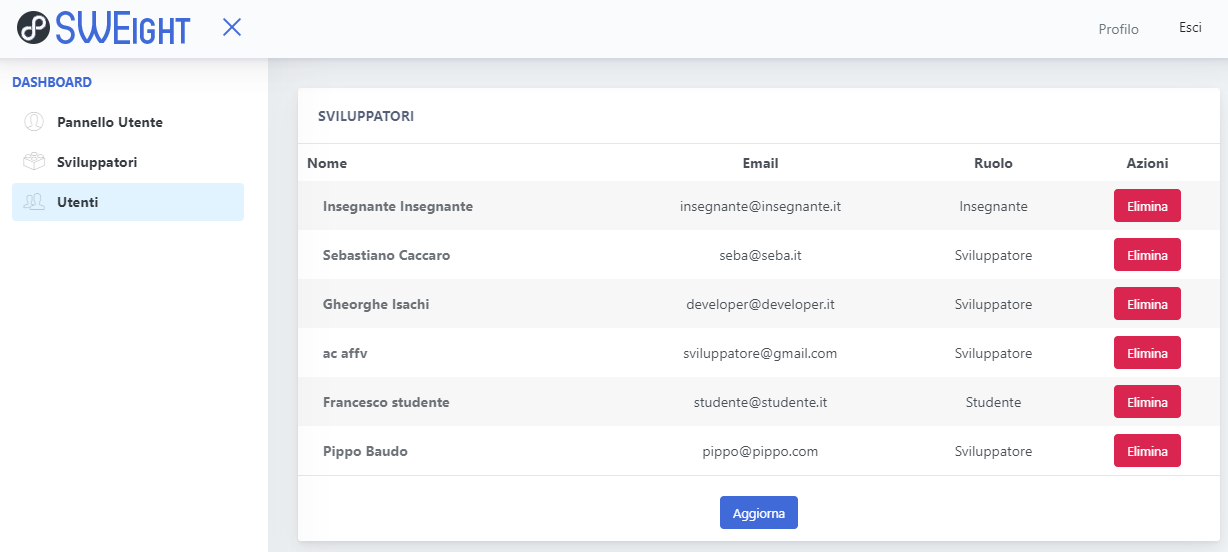
\includegraphics[width=17cm]{sez/img/amministratore/gestisciutenti.PNG}
				\caption{Gestione utenti}\label{fig:1}
			\end{figure}
		  In questa pagina l'amministratore può visualizzare gli utenti iscritti ed eventualmente eliminarli dal sito. Per ogni utente sono presenti Nome, email e ruolo (Insegnate, Sviluppatore o Allievi). Gli amministratori non figurano in questo elenco. L'amministratore, cliccando su \textit{Elimina}, può cancellare un utente dal sistema. Premendo su \textit{Aggiorna}, l'amministratore aggiorna la lista di utenti.
